I sistemi distribuiti funzionano tramite lo scambio di messaggi tra processi situati su nodi diversi, eterogenei e distribuiti geograficamente.\\
Quali sono i modelli di comunicazione?

\section{Middleware Protocols}
Il middleware è un livello che fonde sessione e presentazione della pila ISO/OSI e contiene i servizi di comunicazione di alto livello: socket, remote procedure call, ecc.\\
Nel middleware ci sono sistemi di protocolli che definiscono servizi utili per un ampio spettro di applicazioni (authentication, locking, commit distribuito ad esempio).

\section{Tipi di comunicazione}
Adottiamo modello client server, dove anche il client può fungere da server. 
\begin{center}
    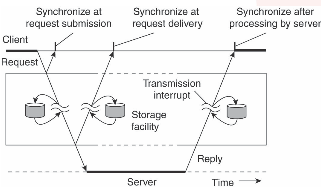
\includegraphics[width = .6\textwidth]{images/lezione3/tipicomunicazione.png}
\end{center}
Analizziamo la foto: da sinistra a destra scorre il tempo. \\
Il client è in esecuzione, fa una richiesta al server, con una certa latenza (rappresentata dall'inclinazione della freccia). È possibile che questa richiesta parta e attraversi un sistema che fornisce memorizzazione (es. mando SMS e questo viene memorizzato in server SMS e se il server non è disponibile, lo riceve dopo).\\ 
Il client potrebbe chiedere una sincronizzazione a livello di invio della richiesta, sincronizzazione a  ricezione della richiesta, oppure sincronizzazione che il server ha effettivamente processato la richiesta. \\
Ci sono quindi vari tipi di sincronizzazione con il server.

\section{Persistenza e sincronia nella comunicazione}
Insieme di post office nei quali la posta viene trasferita tra i vari post office e se il destinatario non è disponibile riesce comunque a rimediare le sue lettere grazie al post office di riferimento. \\
Viene introdotto così un sistema di memorizzazione intermedio. \\
La comunicazione può essere anche transiente ossia in completa assenza di metodi per memorizzare messaggi in transito (una telefonata, ad esempio, senza segreteria telefonica)\\

Abbiamo diverse combinazioni di queste dimensioni:
\begin{itemize}
    \item Persistente asincrono: processo A (in esecuzione) manda un messaggio al processo B (non in esecuzione), c'è un metodo di memorizzazione intermedio che salva il messaggio. A non aspetta nessun ack da B, e va avanti a lavorare.
    \item Persistente sincrono: processo A manda messaggio, B manda conferma (anche se non era in esecuzione), A attende conferma.
    \item Transiente asincrono: A manda messaggio e continua l'esecuzione, il messaggio può essere inviato solo se B è in esecuzione.
    \item Transiente sincrono: 
    \begin{itemize}
        \item Receipt-based: A manda messaggio e si ferma (aspetta conferma), B è in esecuzione ma sta facendo altro, B comunica che l'ha ricevuto (anche se non lo sta elaborando)
        \item Delivery-based: si differenzia dal precedente nel momento di sincronizzazione. Tiene A fermo fino a quando non comncia a dare effettivamente attenzione la richiesta.
        \item Response-based: è il più comune. Non c'è meccanismo di persistenza. B deve essere attivo. A si ferma finché non riceve il risultato di elaborazione della richiesta.
    \end{itemize}
\end{itemize}


\section{Communication middleware}
\subsection{Message oriented transient communication}
Socket introdotte con la versione Berkley di Unix.\\
È un metodo di comunicazione che si appoggia al livello di trasporto (sta sopra). Ha avuto un grandissimo successo ed è passato su tutte le piattaforme. \\
Oggi sono molto diffuse le web socket, ma tutto deriva da questo modello di base.\\

Con socket si intende un estremo del canale di comunicazione (ci sarà una socket per il client e una per il server).\\
Scrivendo programmi con linguaggi a basso livello (C) abbiamo a disposizione diverse primitive:

% TABELLA MULTILINEA
\begin{table}[!h]
    \centering
    \begin{tabular}{|p{.12\textwidth}|p{.70\textwidth}|}
        \hline
         Primitiva & Significato \\
        \hline
          Socket & Crea un nuovo endpoint di comunicazione, a livello di s.o. crea uno spazio di memoria e ci associa un numero\\ 
          \hline
          Bind &  Associa una porta del nodo locale ad una socket\\
          \hline
          Listen & Comando che esegue solo il server: annuncia la dipsponibilità di accettare connessioni \\ 
           \hline
          Accept & Comando che esegue solo il server: blocca il chiamante fino a quando non arriva una richiesta di connessione  \\ 
          \hline
          Connect & Comando che esegue solo il client: avrà come argomenti ip e porta, che corrispondono all'ip del nodo dove sta il server e la porta della socket del server.\\ 
          \hline
          Send & Invio dati nel canale.\\
          \hline
          Receive & Ricevo dati dal canale.\\
          \hline
          Close & Comando da non dimenticare: rilascia le risorse allocate dal sistema operativo (file descriptor, aree di memoria).\\
        \hline
    \end{tabular}
\end{table}
\begin{center}
    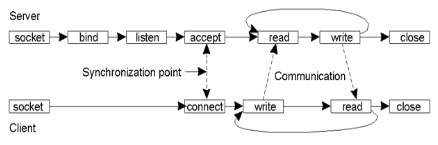
\includegraphics[width = .7\textwidth]{images/lezione3/berkley-socket.png}
\end{center}
Come possiamo vedere dallo schema sia client che server creano una socket. \\
La bind lato client viene fatta in modo implicito dal sistema operativo.\\
Il server fa esplicitamente la bind perché si potrebbe voler usare una porta specifica (mettendo 0 viene scelta una porta qualsiasi, la prima disponibile). \\
La listen dice al sistema operativo di riservare un'area di memoria in cui posso accodare le richieste, poiché non voglio che queste vengano rifiutate se il server è già impegnato. Gli viene data anche una dimensione di quest'area (quante richieste accodare) e se arrivano altre richieste oltre a quel numero, vengono rifiutate. \\
La accept prende il primo elemento (FIFO) nella coda della listen e stabilisce la connessione con questo. La accept restituisce un altro socket descriptor (socket di servizio).\\
Questo server viene implementato come multi-thread, quindi la socket di servizio sarà dedicata alla comunicazione con il client da parte di un thread e la socket principale viene lasciata a gestire le altre richieste. \\
Dopodiché c'è un ciclo di read e write, come se scrivesse su un file. \\
Alla fine della comunicazione sarebbe meglio rilasciare le risorse esplicitamente, altrimenti ci pensa sistema quando viene chiuso il processo.\\

Il modello delle socket è sincrono. \\
Il server esegue una accept per accettare le connessioni da parte del client che rimane bloccato fino a quando non arriva una connessione. \\
Il client che esegue una connect deve trovare dall'altra parte il server pronto a rispondere sulla porta sulla quale sta richiedendo la connessione. \\
Se la connect non trova il server c'è un timeout per cui dopo un tot dà errore. Il client rimane bloccato finché non riesce a fare questa operazione.

\subsection{Message Oriented Persistend Communication: Sistemi di code}
Modello di comunicazione persistente, sempre message oriented.\\ I sistemi che più vengono utilizzati in questi caso sono i sistemi a code. Si hanno due nodi, un sender e un receiver. Ognuno ha un proprio OS, una connessione di rete, con tutti gli stack di protocolli. A livello middleware c'è uno strato, il queuing layer, dove vengono gestite delle code. \\
Dal lato local OS c'è un punto di comunicazione nel server e nel receiver che sono un punto di accesso alle code e non più alla socket del processo. \\
Da parte del codice del server e del receiver il riferimento per inviare e ricevere i messaggi è un punto d'entrata al middleware delle code.
\begin{center}
    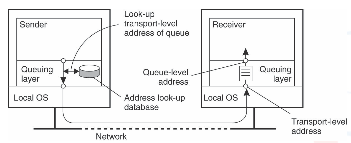
\includegraphics[width = .7\textwidth]{images/lezione3/message-queue.png}
\end{center}
Spesso questo sistema delle code, per implementare la persistenza in modo più affidabile, fa riferimento a nodi intermedi identificati come routers. In pratica viene utilizzato il sistema visto per il pony express: una serie di "uffici postali" intermedi che si occupano dell'instradamento e della gestione dei messaggi per consegnarli al ricevente finale che potrebbe non essere in esecuzione. Questo garantisce persistenza.\\
Il sender manda un messaggio a una coda che fa riferimento al sistema di routing intermedio e arriverà all'applicazione ricevente tramite una coda alla quale saranno recapitati i messaggi.

\begin{table}[!h]
    \centering
    \begin{tabular}{|p{.12\textwidth}|p{.70\textwidth}|}
        \hline
         Primitiva & Significato \\
        \hline
          Put & esegue l'append di un messaggio a una coda specifica \\ 
          \hline
          Get & preleva i messaggi da una coda. È una primitiva bloccante: si blocca fin quando trova un elemento. Se c'è più di un elemento utilizza una politica FIFO\\
          \hline
          Poll & è una get non bloccante. Preleva il primo messaggio presente senza mai bloccare l'esecuzione\\ 
           \hline
          Notify & installa un handler che può essere chiamato quando un messaggio viene messo nella coda specificata. (Una specie di trigger che può servire per fare l'opposto della poll dall'altra parte) \\ 
        \hline
    \end{tabular}
\end{table}


\subsubsection{Message Brokers}
Il ruolo dei broker in un message queue system non è soltanto quello di garantire la persistenza nel caso in cui i nodi riceventi siano offline, oppure i processi non siano disponibili, ma potrebbe dover fare delle traduzioni/conversioni. \\
\begin{center}
    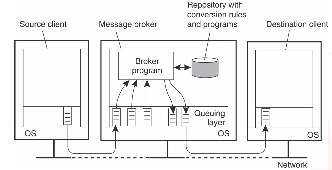
\includegraphics[width = .7\textwidth]{images/lezione3/broker.png}
\end{center}
I nodi in un sistema distribuito possono essere eterogenei e potrebbe essere utile inserire in questo middleware anche un metodo per far parlare nodi che hanno convenzioni diverse.\\
Il broker oltre a gestire le code per ingresso/uscita di messaggi, potrebbe avere accesso a una repository con delle regole di conversione (traduzioni) da utilizzare per tradurre i messaggi nel caso in cui i due nodi utilizzino standard diversi.\\

\textbf{Quando conviene usare i sistemi a code?}\\
Conviene usare un sistema a code quando:
\begin{itemize}
    \item si deve implementare comunicazione asincrona con persistenza
    \item quando la scalabilità può aumentare ammettendo ritardi in risposte e richieste
    \item quando il producer è più veloce del consumer
    \item quando si implementa il pattern di comunicazione publish subscribe
\end{itemize}

\subsubsection{Protocolli di messaging}
I protocolli a messaggi più comuni sono:
\begin{itemize}
    \item \textbf{XMPP}: utilizzato in precedenza da Google Talk e FB fino al 2014. È basato su XML e permette di strutturare con i tag i contenuti dei messaggi. Supportava la presence information, cioè capire quando un utente è collegato e dare un ack a chi deve comunicare per vedere chi è presente o no, manutenzione di contact list, ecc. Era aperto. 
    \item \textbf{MQTT}: sviluppato da IBM con l'intenzione di creare qualcosa di leggero. L'obiettivo finale era quello di riuscire a far utilizzare questo protocollo anche a client estremamente thin, quindi anche dispositivi IoT. Questi protocolli lavorano sopra TPC/IP. Ogni client ha un ID univoco. MQTT in generale non garantisce persistenza. È stato creato per il modello publish subscribe. Il broker gestisce la coda. Ci sono altri client che si registrano al broker dicendo che vogliono i dati che vengono pubblicati su una certa coda. Usato da FB Messenger. Utilizza lo standard OASIS ed è uno dei principali candidati per comunicazione machine to machine in ambito IOT.
    \item \textbf{AMPQP}: utilizza lo standard ISO. Perfetto per un'ampia gamma di infrastrutture middleware di messaggistica e anche
per il trasferimento dei dati peer-to-peer.
\end{itemize}

\subsubsection{Message broker software}
I principali software dei message brokers sono:
\begin{itemize}
    \item Eclipse Mosquitto: supporta MQTT, è leggero e opensource
    \item RabbitMQ: molto popolare, opensource e supporta AMQP e altri protocolli
    \item Apache ActiveMQ and Kafka
    \item Google Cloud Pub/Sub
    \item Amazon MQ
\end{itemize}

\paragraph{RabbitMQ}
È un'implementazione multi-linguaggio dell'AMQP, ma supporta plugin per MQTT ed altro protocolli. Consiste in:
\begin{itemize}
    \item un broker (distribuito in un cluster o in un insieme di cluster), scritto in Erlang
    \item client disponibili per vari linguaggi e i client comunicano con il broker utilizzando AMQP
\end{itemize} 
\begin{center}
    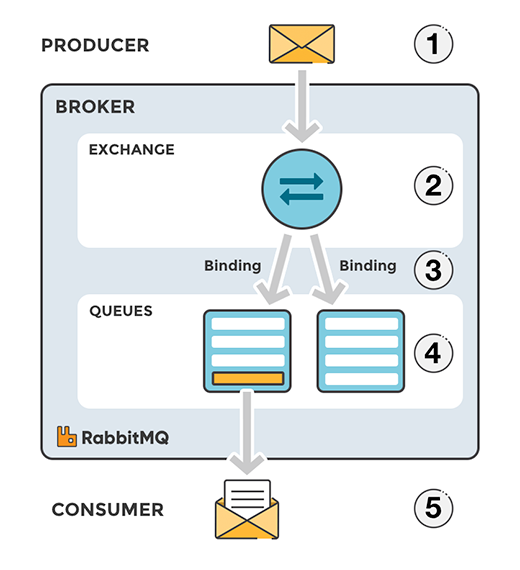
\includegraphics[width = .5\textwidth]{images/lezione3/rabbitmq.png}
\end{center}
Il message flow classico è: il producer (publisher) manda i dati che produce al broker (nella parte di gestione dei producer), in cui viene rediretto il messaggio a determinate code e dalle code viene instradato verso i consumer (subscriber). \\
RabbitMQ ha molte funzionalità: per esempio supporta la modalità diretta, cioè il messaggio contiene una chiave/stringa che lo direziona verso una sola coda specifica alla quale c'è un consumer specifico. Questo è un modo per rendere asincrona e persistente una comunicazione 1:1 come quella client-server. \\
Oppure c'è la funzione opposta in cui il messaggio viene mandato a tutti. \\
La modalità più usata, anche in MQTT, è invece che il producer pubblica il messaggio specificando un "topic". Ci sono code dedicate a questi "topic" e serve un sistema estremamente efficiente per gestire tutti i subscriber che si iscrivono ad un determinato "topic". \\
Il passaggio dei dati ai consumer (subscriber) funziona in questo modo: il subscriber si registra al sistema (al broker), ottiene un identificatore e stabilisce una connessione. Nel registrarsi al broker, il processo consumer che gira su un nodo stabilisce una connessione con il broker (esattamente come per la socket) e questa connessione viene poi utilizzata per mandargli i messaggi di sua competenza. \\
Nel caso in cui il consumer vada offline, chiuda la connessione o ci sia un problema di rete, il sistema deve prevedere dei modi affinché se riprende la connessione e il consumer è registrato già con un certo ID, viene riconosciuto e ricomincia la trasmissione su un nuovo canale. \\

\section{Remote Procedure Call}
Le Remote Procedure Call sono un metodo per introdurre trasparenza di accesso rispetto alla comunicazione via messaggi.
L'obiettivo è avere un modo per scrivere programmi (come siamo abituati a scriverli) sul sistema distribuito, senza esplicitare canali tra processi.\\
Vogliamo comunicare con altri perchè magari alcune operazioni non le sa fare il mio nodo, ma uno più potente sì. 
RPC nasconde la messaggistica che è necessaria per simulare una chiamata a procedura remota.

\subsection{Chiamata a procedura convenzionale}
Abbiamo una procedura read(fd, buf, nbytes). Durante la sua esecuzione si popola lo stack mano a mano che si eseguono le istruzioni.\\
Ad una procedura locale possiamo passare i parametri per:
\begin{itemize}
    \item valore
    \item riferimento
\end{itemize}
Ovviamente non possiamo usare il passaggio per riferimento per una RPC, perchè l'indirizzo di memoria sulla mia macchina sarà diverso rispetto alla macchina remota. Si deve serializzare e passare per valore.\\ Se ho una grossa mole di dati, questo è molto costoso. 

\subsection{Client e Server Stubs}
Lato client è come se chiamassi una procedura locale, il middleware si occuperà di tradurre tutto in una richiesta, in una chiamata alla procedura sul server, e alla restituzione del risultato. 
\begin{center}
    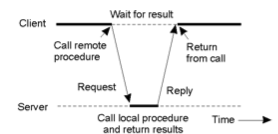
\includegraphics[width = .5\textwidth]{images/lezione3/clientserverstub.png}
\end{center}

\subsection{Passi di una RPC}
Sul client abbiamo le varie istruzioni e ad un certo punto nel codice c'è una chiamata ad una funzione che vogliamo far eseguire sul server. \\
Qui interviene un pezzo di codice che è stato automaticamente generato che non è visto dal programmatore. \\
All'interno di questa porzione di codice abbiamo la serializzazione dei parametri e l'invio di questi come messaggio (costruito dallo stub).\\
Dall'altra parte del canale di trasmissione c'è la risalita di tutti i livelli della pila ISO/OSI fino ad arrivare al processo che si è reso disponibile per eseguire quella funzione. \\
Il server ha un codice che implementa la funzione richiesta, che un programmatore ha scritto, non per rispondere a richieste di altri dall'esterno, ma per eseguire questa funziona in locale.\\
C'è però come nel client una porzione di codice stub che fa il lavoro di spacchettare il messaggio, costruire la struttura dati, identificare la funzione e fare la chiamata alla funzione come se fosse una chiamata locale.\\
Il risultato verrà preso dallo stub, messo in un messaggio, e inviato dall'altra parte.\\
Il client ricostruisce il risultato e riprende la sua esecuzione.\\
Le stub del client e quelle del server possono essere scritte in linguaggi diversi.

\subsection{Marshalling e Unmarshalling}
Sono due procedure, una opposta all'altra:
\begin{itemize}
    \item Marshalling: formattazione dei parametri di una RPC in un messaggio
    \item Unmarshalling: estrarre i parametri dal messaggio
\end{itemize}
Il Marshalling richiede la serializzazione degli oggetti o delle strutture dati (codifica in sequenza di byte che può essere inviata sul canale).\\
La serializzazione può essere effettuata in binario (come nelle Java RMI o in gRPC) o in stringhe (ad esempio REST WS in JSON).\\

\textit{Se sono in un sistema eterogeneo i nodi interpretano le cose in modo diverso.}

\subsection{RPC sincrone e asincrone}
Tipicamente RPC è sincrona. È possibile però chiedere anche una chiamata asincrona, eventualmente, con dei parametri. \\
C'è la possibilità di ricevere ack a chiamata ricevuta, oppure con la modalità deferred synchronous, si aspetta un tot fino all'accettazione della richiesta, ma non si aspetta il risultato e si continua a lavorare. \\
One-way RPC non chiede di eseguire niente al client e il client semplicemente manda un ack. (modalità quasi asincrona)

\subsection{Scrivere un client e un server}
\begin{center}
    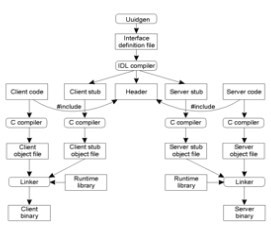
\includegraphics[width = .5\textwidth]{images/lezione3/writingrpc.png}
\end{center}
Il server per pubblicare metodi remoti deve scrivere una interfaccia in IDL. Caratteristiche di una IDL (deve essere scritta in un linguaggio neutro - esistono piu` compilatori in base al linguaggio che si vuole ottenere, questi compilatori, dato l’IDL creano automaticamente Server e Client Stub):
\begin{itemize}
    \item Come si chiama il metodo
    \item Parametri e tipo del metodo
\end{itemize}
 
\subsubsection{gRPC}
gRPC è un'implementazione di Google del protocollo RPC. È un framework open source, usato largamente per la sua caratteristica di avere una bassa latenza e un'alta scalabilità all'interno dei sistemi distribuiti. Supporta molti linguaggi di programmazione come C,C++, Java, Python, Go ...\\
In gRPC viene usato ProtoBuf per la comunicazione.


\subsection{Associare un client a un server}
In un sistema distribuito sarebbe opportuno anche avere trasparenza rispetto alla location. \\
In Corba c'è un modo per scoprire dinamicamente chi è disposto a offrire certe funzioni. Dal punto di vista del programmatore è possibile interrogare un server directory e avere in restituzione l'indirizzo di un nodo che in quel momento è disponibile per quella funzione.
\begin{center}
    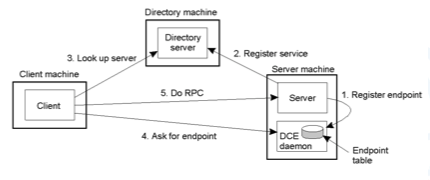
\includegraphics[width = .7\textwidth]{images/lezione3/bindingclientserver.png}
\end{center}
Lato server machine viene comunicato a un processo demone a quale porta si risponde e viene pubblicato il servizio sul directory server. \\
Il client fa una ricerca di chi offre la funzionalità attraverso il directory server che gli fornisce la porta e l'indirizzo ip del demone sul nodo (non indirizzo del server specifico).\\
Successivamente il client chiede al demone sulla server machine l'endpoint della server stub. \\
Il demone guarda se sulla sua macchina qualcuno offre quella funzione, verifica se è il servizio è attivo e se non lo è, lo lancia. \\
A questo punto il servizio è attivo e gli restituisce la porta. \\
Finalmente il client può eseguire una RPC. \\


\begin{comment}

FABBIO

Il sistema distribuito funziona tramite scambio di messaggi tra processi in esecuzione su nodi diversi anche eterogenei.

Middleware protocol:
Sopra al livello trasporto. Possono essere collocati i servizi di alto livello tipo socket, remote procedure call...
SOno un sistema di protocolli che
definisce servizi utili per un ampio spettro di applicazioni tipo autenticazione, protocolli di commit per transazioni....
[Ripetizione a sinistra e a destra dei quadrati perchè rappresentano due nodi.]

Tipi di comunicazione:
Persistenza: si ha un sistema di server che aiuta in questo processo di EH....
Transiente: quando non c'è nessun metodo per memorizzare nessun messaggio in transito. QUindi se non c'è il server pronto a ricevere non si fa niente. Tipo chiamata, se è occupato non riesci a fare la chiamata.

Persistenza e sincronity nella comunicazione:
\textit{persistente-asincrono}: forse il più difficile da implementare. Processo A manda un messaggio a B e B non è in esecuzione. C'è un metodo di memorizzazione intermedia e A non aspetta nessun ack di conferma. B quando torna disponibile farà l'operazione richiesta da A
\textit{persistente-sincrono}: Come quello precedente ma A aspetta l'ack di conferma. L'ack di conferma dice semplicemente che la richiesta è stata ricevuta (non processata).

\textit{transiente-asincrona}: come la prima ma non c'è memorizzazione intermedia
\textit{transiente-asincrona}: B è in esecuzione ma sta facendo altro. B può ricevere e inviare l'ack di conferma. A si ferma fino a che non ha ricevuto l'ack di conferma che la richiesta è stata presa in carico da B.

\textit{Delivery-based transient}:
\textit{response-based transient}: 

Communication middleware:
Berkeley sokets:
Sta sopra a livello di trasporto e da unix è passato a tutte le piattaforme. Usando le socket in C si hanno le visibilità delle primitive di sistema e quindi si può capire cosa avviene nel sistema operativo.
Per socket si intende l'estremo di un canale di comunicazione. 
La primitiva socket crea un end point che dovrà essere eseguita sia dal client sia dal server.
Dal punto di vista del sistema operativo (riferimento a unix) crea un descrittore che sta nello spazio del processo (è privato al processo). In un sistema unix i file descrittor sempre presenti sono standard I/O error. (0, 1, 2, 3).32
...

Message oriented persistent communication: queuing systems
Sempre message oriented ma con un meccanismo di persistena.
Sistemi più utilizzati sono i sistemi a code. A livello di middlewere c'è uno strato di queuing layer. 

Message queuing systems with routers:
Message-queuing Model
Message brokers: 


Messaging protocols:
XMPP: usato da facebook era implementata con XMPP. Basato su XML. Supportava il discorso della present information per capire quando un utente è collegato. Era aperto....
MQTT....
AMQP:
Standard ISO. Advanced perchè permette più funzionalità di MQTT. Fa più cose di MQTT.

------------------------------------------------------
Virgola, il gattino

Sistema distribuito funziona tramite scambio di messaggio tra processi in escuzione su nodi diversi, eterogenei e distribuiti geograficamente. 
Si comunica a basso livello su canali tra i nodi (?).

Sessione e presentazione sono fusi in un livello di middleware. Il corso tratta ciò che sta sopra al livello di trasporto. Nel middleware possono essere collocati i servizi di comunicazione di alto livello: socket, rpc, ecc. I protocolli di middleware sono un sistema di protocolli che definisce servizi utili per un ampio spettro di applicazioni (es. autenticazione, locking, commit distribuito (?)).

Tipi di comunicazione:
DISEGNO
Da sinistra a destra scorre il tempo. Il client è in esecuzione, fa una richiesta al server, con una certa latenza. È possibile che questa richiesta parta e attraversi un sistema che fornisce memorizzazione (es. mando SMS e questo viene memorizzato in server SMS e se il server non è disponibile, lo riceve dopo). Quindi, un meccanismo di memorizzazione intermedio. Il client potrebbe chiedere una sincronizzazione a livello di invio della richiesta, sincronizzazione a  ricezione della richiesta, oppure sincronizzazione che il server ha effettivamente processato la richiesta. Ci sono quindi vari tipi di sincronizzazione con il server.

Persistenza e transienza.
Persistente, esempio del pony express. Se il destinatario non è disponibile, riesce comunque ad ottenere la sua posta dal post office di riferimento.
Transiente non c'è nessun metodo per memorizzare i messaggi in transito. Se il server non è disponibile a ricevere, non è possibile svolgere la comunicazione.

Caso a: 
offre diversi vantaggi. Il processo A in esecuzione manda un messaggio al processo B. B non è in esecuzione. C'è un metodo di memorizzazione intermedia. È asincrono perché A non aspetta nessun ack ne dall'infrastruttura ne da B. 
Caso b:
ci possono essere diversi livelli di (a)sincronicità. A in questo caso non continua a lavorare, riprende quando arriva l'ack che conferma l'accettazione della richiesta. B non era in esecuzione, ma sul nodo B c'è un qualche processo almeno in grado di accettare la richiesta. Ha persistenza perché il processo target non era in esecuzione, eppure è andato a buon fine. È sincrono perché si ferma.
Caso c:
A manda un messaggio e B deve essere attivo. L'assenza di memorizzazione intermedia dice che è transiente. Il fatto che A continua indica che è asincrono.
Caso d:
Questo esempio è transiente e sincrono. Diversi livelli di sincronicità. B è in esecuzione, ma sta facendo qualcos'altro. È possibile allocare al processo una coda che accetta richieste in una certa del sistema operativo allocata a questo processo, quindi anche se sta facendo qualcos'altro è possibile ricevere e accodare le richieste. B andrà a prendere in quest'are temporanea del processo B i messaggi arrivati e li gestirà. La parte sincrona è che A si ferma finché non ricevuto un ack.
Caso e:
si differenzia dal precedente nel momento di sincronizzazione. Tiene A fermo fino a quando non comncia a dare effettivamente attenzione la richiesta.
Caso f: 
il più comune. Non c'è meccanismo di persistenza. B deve essere attivo. A si ferma finché non riceve il risultato di elaborazione della richiesta.

Berkeley Sockets: sono state introdotte con la versione di UNix chiamata Berkeley Unix. Si appoggia al livello di trasporto (sta sopra). Ha avuto grandissimo successo ed è passato su tutte le piattaforme. Oggi sono diffuse le web socket. Tutto deriva da questo modello di base.

Primitive sistema comunicazione con socket:
- Con socket si intende l'estremo di un canale di comunicazione. Quante ne servono? 2. Sia client che server creano la socket. Dal punto di vista del sistema operativo (unix) questa cosa crea un descrittore che sta nello spazio (privato) del processo. Standard input, standard output e standard error sono 3 descrittori base che vengono creati alla creazione del processo (?).  
- Bind fa si che una socket sia associata ad una porta. La porta è unica per tutto il nodo, al contrario dei file desdcriptor.
- Listen la fa solo il server. Annuncia la disponibilità ad accettare connessioni.
- Accept è bloccante.  La fa il server.
- Connect la fa il client, una volta che ha la socket descriptor e ha associato una porta. La primitiva connect avrà come argomenti ip e porta, che corrispondono all'ip del nodo dove sta al server e la porta della socket del server.
- Dopodiché posso fare un ciclo di send e receive a piacere.
- Close, non va dimenticata. Rilascia le risorse (file descriptor, aree di memoria allocati dal sistema operativo).

Entrambi creano una socket. La bind lato client viene fatta in modo implicito dal sistema operativo. Il server fa esplicitamente la bind perché potrei volere una porta specifica. Mettendo 0 mette una porta qualsiasi, la prima disponibile. La listen dice al SO di riservare un'area di memoria in cui posso accodare le richieste, poiché non voglio che vengano rifiutato le richieste, se sono già impegnato. Gli do anche una dimensione di quest'area (quante richieste accodare) oltre a quel numero, vengono rifiutate le richieste. La accept prende il primo elemento FIFO nella coda della listen e stabilisce la connessione con questo. La accept restituisce un altro socket descriptor (socket di servizio). Questo server viene implementato come multi-thread, quindi la socket di servizio sarà dedicata alla comunicazione con il client da parte di un thread e la socket principale viene lasciata a gestire le altre richieste. Dopodiché c'è un clico di reat e write, come se scrivesse su un file. Alla fine sarebbe meglio rilasciare le risorse, altrimenti ci pensa sistema quando viene chiuso il processo.

Il modello delle socket è sincrono. Il server esegue una accept per accettare le connessioni da parte del client che rimane bloccato fino a quando non arriva una connessione. Il client che esegue una connect deve trovare dall'altra parte il server pronto a rispondere sulla porta sulla quale ha fatto la connessione. Se la connect non trova il server c'è un timeout per cui dopo un po' dà errore. Il client è fermo finché non riesce a fare questa operazione.

Queuing Systems
Modello di comunicazione persistente, sempre message oriented. I sistemi che più vengono utilizzati in questi caso sono i sistemi a code. Due nodi, un sender e un receiver. Ognuno ha un proprio OS, una connessione di rete, con tutti gli stack di protocolli. A livello middleware c'è uno strato queuing layer dove vengono gestite delle code. Dal lato local OS c'è un punto di comunicazione nel server e nel receiver che sono un punto di accesso alle code e non più la socket del processo. Da parte del codice del server e del receiver il riferimento per inviare e ricevere i messaggi è un punto d'entrata al middleware delle code.

Spesso questo sistema delle code per implementtare la persistneza in modo più affidabile fa riferimento a noid intermedi identificati come routers. Utilizza il sistema visto per il pony express: una serie di "uffici postali" intermedi che si occupano dell'instradamento e della gestione dei messaggi per consegnarli al ricevente finale che potrebbe non essere in esecuzione. Questo garantisce persistenza.

Il sender manda messaggio a una coda che fa riferimento al sistema di routing intermedio e arriverà all'aplpicazione ricevente che legge da una coda alla quale saranno recapitati i messaggi.

Primitive: (nomi diverse nei vari linguaggi di programmazione)
- Put manda un messaggio. Fa append a una coda.
- Get su una certa coda, prende i messaggi. È una primitiva bloccante, si blocca fin quando trova un elemento. Se c'è più di elemento usa politica FIFO.
- Poll, get non bloccante. Il codice esegue altre istruzione, ma verifica periodicamente se nella coda ci sono messaggi da gestire, senza bloccarsi.
- Notify, trigger che può servire per fare l'opposto della poll dall'altra parte

Il ruole dei broker in un message queue system non è soltanto quello di garantire la persistenza nel caso in cui i nodi riceventi siano offline, oppure i processi non siano disponibili. Il broker potrebbe fare delle traduzioni/conversioni. I nodi in un sistema distribuito possono essere eterogenei e potrebbe essere utile inserire in questo middleware anche un metodo per far parlare nodi che hanno convenzioni diverse. Il broker oltre a gestire le code per ingresso/uscita di messaggi, potrebbe avere accesso a una repository con delle regole di conversione se i due nodi utilizzano standard diversi per riuscire a rendere trasparente l'accesso.

Quando un sistema a code è preferibile ad un sistema di comunicazione sincrona?
- Quando mi accorgo che ho bisogno di comunicazione asincrona e persistente
- Se ammetto ritardi nella gestione di richieste / trasmissione rete (?)
- Il sender è magari un sensore che produce molti dati ad altra frequenza e il consumatore non riesce a gestirli tutti
- Quando si implementa un pattern publish-subscribe

Le code sono legate ad una specifica applicazione o sono legate ad un nodo? Dipende dal sistema a code che si va ad installare. A volte sono gestite addirittura da un broker fuori dal nodo, ma di solito sono condivise. 

Protocolli a messaggi più comuni:
- XMPP: utilizzato in precedenza da google talk e FB fino al 2014. È basato su XML e permette di strutturare con i tag i contenuti dei messaggi. Supportava la presence information, cioè capire quando un utente è collegato e dare un ack a chi deve comunicare per vedere chi è presente o no, manutenzione di contact list, ecc. Era aperto. 
- MQTT: sviluppato (da IMB?) con l'intenzione di creare qualcosa di leggero. Riuscire a far utilizzare questo protocollo anche a client estremamente thin, quindi anche dispositivi IoT. Questi protocolli lavorano sopra TPC/IP. Ogni client ha un ID univoco. MQTT in generale non garantisce persistenza. È stato creato per il modello publish subscribe. Quello che manda è un produttore di dati e pubblica i dati che produce. Il broker gestisce la coda. Ci sono altri client che si registrano al broker dicendo che vogliono i dati che vengono pubblicati su una certa coda. Usato da FB Messenger. OASIS standard ed è uno dei principali candidati per comunicazione machine to machine in ambito IOT.
- AMPQP: standard ISO. Permette molte più funzionalità di MQTT, ma consente anche di fare le stesse cose.

Eclipse Mosquitto supporta MQTT. Altro software di message queuing estremamente popolare è RabbitMQ. Tanti altri sistemi in ambito cloud: Amazon MQ, Apache ActiveMQ, ecc. (?)

RabbitMQ:
ci si può connettere a questo sistema da moltissimi linguaggi di programmazione. È un'implementazione dell'AMQP, ma ha plugin per MQTT ed altro protocolli. Consiste in un broker (distribuito in un cluster o in un insieme di cluster), è scritto in Erlang. Ci sono client disponibili per vari linguaggi e i client comunicano con il broker utilizzando AMQP. Il message flow classico è: abbiamo il producer (publisher) che manda i dati che produce al broker nella parte di gestione dei producer, in cui viene rediretto il messaggio a determinate code e dalle code viene instradato verso i consumer (subscriber). Ha molte funzionalità, per esempio supporta la modalità diretta, cioè il messaggio contiene una chiave/stringa che lo direzione verso una sola coda specifica alla quale c'è un consumer specifico e potrebbe essere dedicata. Questo è un modo per rendere asincrona e persistente una comunicazione 1:1 come quella client-server. Oppure c'è l'opposto in cui il messaggio viene mandato a tutti. La modalità più comunque, usata anche in MQTT, è invece che il producer pubblica il messaggio specificando un "topic". Ci sono code dedicate a questi topic e serve un sistema estremamente efficiente per gestire tutti i subscriber che si iscrivono ad un determinato topic. Il passaggio dei dati ai consumer (subscriber) funziona in questo modo: il subscriber si registra al sistema (al broker), ottiene un identificatore e stabilisce una connessione. Nel registrarsi al broker, il processo consumer che gira su un nodo stabilisce una connessione con il broker (esattamente come per la socket) e questa connessione viene poi utilizzata per mandargli i messaggi di sua competenza. Nel caso in cui il consumer vada offline, si chiuda la connessione o c'è un problema di rete, il sistema deve prevedere devi modi affinché se riprende la connessione e il consumer è registrato già con un certo ID, viene riconosciuto e ricomincia la tramissione su un nuovo canale. Oppure ci sono metodi tipo push in cui il server manda al consumer ... (?). Ci sono varie modalità a seconda del sistema di message queuing. Non c'è una coda per ogni consumer.

Remote Procedure Call
Un metodo per introdurre trasparenza di accesso rispetto alla comunicazione via messaggi. Vorremmo riuscere a fare (cosa???) senza dover esplicitamente stabilire questi canali con gli altri processi. Perché? Potrebbe esserci qualche nodo con una potenza di calcolo maggiore e la lancio su quello. Vorremmo che fossero chiamate in locale (senza che il programmatore si debba preoccupare di dove vengono eseguite) e invece vengono eseguite in remoto. Questo è un metodo per introdurre trasparenza di accesso.
Come funziona una rpc standard? Abbiamo una istruzione di read, normalmente allochiamo dello spazio di memoria sullo stack. I parametri non possono essere passati per indirizzo, essendo riferito allo spazio locale del processo. Devono essere serializzati e passati per valore. Se ho una grossa mole di dati, questo è molto costoso. Abbiamo il client che fa la chiamata di procedura remota (nel modello più semplice la chiamata RPC è sincrona), esattamente come se fosse in locale, e il middleware deve fare tutte le operazioni affinché si risolva in una chiamata interna al server della procedura e in una restituzione del risultato, che viene messo nella struttura dati locale.
Sotto sistema operativo con stack tcp/ip, come al solito. Sul client abbiamo le varie istruzioni e ad un certo punto c'è una chiamata ad una funzione che vogliamo far eseguire sul server. A questo punto interviene un pezzo di codice che è stato automaticamente generato, che non è visto dal programmatore. All'interno di questo codice abbiamo una certa modalità di serializzazione dei parametri, di invio come messaggio (lo stub costruisce il messaggio), nella rete viaggia il messaggio opportunamente formattato con i valori e dall'altra parte c'è la risalita di tutti i livelli del protocollo iso/osi fino ad arrivare al processo che si è reso disponibile per eseguire quella funziona ed in fatti ha un codice di implementazione della funzione, che un programmatore ha scritto, ma non per rispondere a richieste di altri dall'esterno. È scritto per implementare questa funziona in locale. C'è però come nel client un pezzo di codice stub che fa il lavore di risponde dal tcp, spacchetta i lmessaggio, costruisce la struttura dati, identifica la funziona lal'interno e fa la chiamate alla funzione come se fosse una chiamata locale. Il risultato verrà preso dallo stub, lo mette in un messaggio, torna dall'altra parte, il client ricostruisce il risultato e il client riprende la sua esecuzione. Lo stub client e server può essere in linguaggi diversi. Java RMI solo stesso linguaggio(?)

Marshalling e unmarshalling:
Processo che lo stub
Marshalling: formatta i programmi della chiamata in un messaggio
Unmarshalling: processo inverso
Marshaling richiede serializzazione degli oggetti o delle strutture dati (codifica in sequenza di byte che può essere inviata sul canale).
La serializzazione può essere effettuata in binario (Java RMI, gRPC) o in stringe (REST WS in JSON).
Uno dei motivi per cui la comunicazione tra microservizi in ambiente container e distribuiti in cloud. La comunicazione deve essere efficiente. In un primo tempo veniva fatto con REST (con JSON). Ultimamente gRPC ha soppiantato, uno dei motivi è la sua maggiore efficienza anche per la codifica binaria della serializzazione e di quello che passa per il canale.

Se sono in un sistema eterogeneo i nodi interpretano le cose in modo diverso. 

Tipicamente RPC è sincrona. È possibile però chiedere anche una chiamata asincrona eventualmente con dei parametri. Possibilità di ricevere ack con chiamata riceveuta oppure modalità deferred syncrhonous, cioè è sincrono, poiché aspetta un pochino fino all'accettazione della richiesta, ma non aspetta il risultato, continua a lavorare. One-way RPC non chiede di eseguire niente al client e il client semplicemente manda un ack. (modalità quasi asincrona)

Chi genera questa poorzione di software? Nei webserver tradizionali c'è un WSDL che generano i client e i server stub. Il problema di generare automaticamente questo codice sta nel capire chi descrive i parametri della procedura. IN una libreria multilinguaggio per RPC (come Corba, gRPC) bisogna avere un linguaggio neutro per definire l'interfaccia delle funzioni. In corba c'è IDL (interface definition language), un linguaggio generale che deve conoscere chi vuole pubblicare e utilizzare delle funzioni e automaticamente da questa specifica con compilatore C genera il binario che viene eseguito dal client (?).

In gRPC c'è ProtoBuf (protocol buffer, analogo JSON) (definizioni finiscono .proto), uno definisce la funzione (nomi e parametri). Dopodiché ho un compilatore (con versione di compilazione, quindi diversi compilatori nella realtà) che compila in diversi linguaggi.

In un sistema distribuito sarebbe opportuno anche avere trasparenza rispetto alla location. In Corba c'è un modo per scoprire dinamicamente chi è disposto a offrire certe funzioni. Dal punto di vista del programmatore è possibile interrogare un server directory, anche senza sapere nome, ma con una descrizione, e avere in restituzione l'indirizzo di un nodo che in quel momento è disponibile per quella funzione.
Comunico a un processo demone a quale porta rispondo e pubblico anche sul directory server. Il client fa una ricerca di chi offre la funzionalità, gli da porta e ip del demone sul nodo (non indirizzo del server specifico) e gli chiede l'endpoint di dove sarà il server stub. Il demone guarda se sulla sua macchina qualcuno offre quella funzione, verifica se è attivo e se non è attivo lo lancia. A questo punto il servizio è attivo e gli restituisce la porta. Finalmente si può fare RPC. C'è un modo per il client di ottenre dinamicamente quel pezzo di codice che permette di fare RPC.


\end{comment}